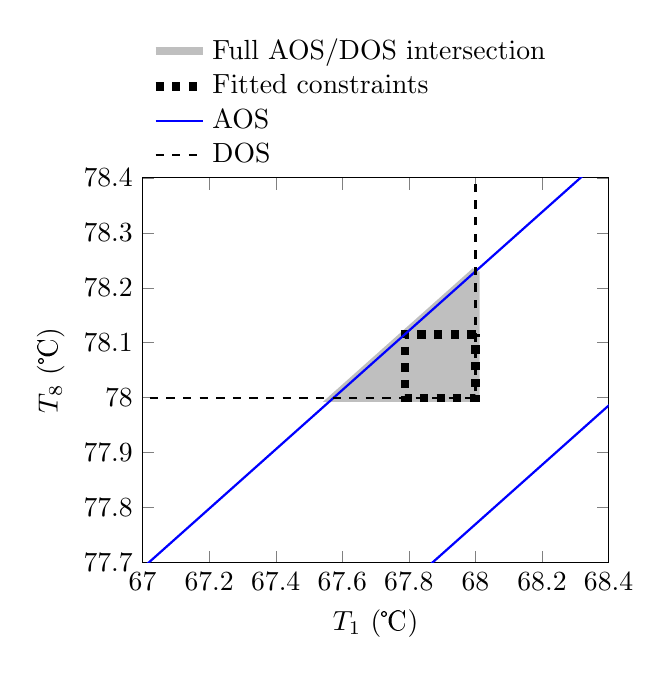
\begin{tikzpicture}
  \begin{axis}[
    width=7.5cm,
    xlabel=$T_1$~(\textcelsius),
    ylabel=$T_8$~(\textcelsius),
    xmin=67,xmax=68.4,ymin=77.7,ymax=78.4,
    xtick={67,67.2,...,68.4},
    ytick={77.7,77.8,...,78.4},
    legend style={
      draw=none,
      at={(0.0,1.0)},
      anchor=south west,
      cells={anchor=west}}]

    %intersection
    \addplot[fill=lightgray,color=lightgray,line width=3pt] coordinates {
      (68.      ,   78.2299483)
      (67.573841,   78.       )
      (68.      ,   78.       )
      (68.      ,   78.2299483)
    };
    %fitted cons
    \addplot[color=black,line width=3pt,dashed] coordinates {
      (67.99999975,  78.11504787)
      (67.78705642,  78.11504787)
      (67.78705642,  77.99999994)
      (67.99999975,  77.99999994)
      (67.99999975,  78.11504787)
    };
   %AOS
    \addplot[color=blue,thick] coordinates {
      (36.685,  60.873) 
      (36.915,  61.457) 
      (99.315,  95.127) 
      (99.085,  94.543) 
      (36.685,  60.873) 
    };
    %DOS
    \addplot[color=black,thick,dashed] coordinates {
      (68,  82)
      (66,  82)
      (66,  78)
      (68,  78)
      (68,  82)
    };
     \legend{Full AOS/DOS intersection,Fitted constraints,AOS,DOS}
  \end{axis}
\end{tikzpicture}
